\documentclass[runningheads]{llncs}
\usepackage{graphicx}
\usepackage{float}
\usepackage{wrapfig}

\usepackage{colortbl}
\graphicspath{ {./images/} }
\begin{document}
\pagestyle{empty}
\title{Enzyme-based digital biosensors for medical applications}
\author{Maren Krafft}
\authorrunning{Maren Krafft}
\institute{Chair of Computer Engineering, University of Passau, Germany}
\maketitle        

      
\begin{abstract}
%es werden nicht biosensors kombiniert
Biocomputing has recently gained a place among other computing paradigms. Utilizing the natural rules of interaction between biochemical substances, mimicking conventional computer systems, new ways and techniques of solving computing problems have been developed. This review covers the concept of digital biosensors, based on enzyme logic networks, that can process multiple biochemical input signals. This concept of utilizing enzymes as the ''machinery'' of biochemical logic networks, aims to create complex analytical biosensors for medical application.


\keywords{Multi-input Biosensors \and Biosensors  \and enzyme-based logic gates \and logic networks \and biomedical applications \and sense-act-treat device \and feedback loop \and transducer \and biocomputing  }
\end{abstract}


\section{Introduction}
%1.Context: what problem is being solved, why relevant or interesting, benefit, possible applications
%2.innovation: described technique completely new or does it improve earlier approcahes? what is improved 
%3.thesolution: how does the presented technique work, core idea of the solution

	In the medical field, digital biosensors (analytic devices to convert the result of a biochemical reaction into an electric signal \cite{definitions}) are an essential tool for the monitoring and detection of a wide range of medical conditions. Biochemical substances are chemical substances that occur in natural environments (e.g.like enzymes or glucose). The currently available sensors work as single-input devices, which can analyse only one specific substance. The new concept aims to create devices that can analyse multiple inputs and transform those into a single output signal. This change allows for a variety of possible applications. \cite{original}\\
	\newline
	Once realized, those biosensors are expected to revolutionize a great number of medical treatments and therapies. Through the analysis of multiple inputs, the sensors could scan specific injuries or diseases. More complex models could create sense-act-treat devices that immediately apply the correct treatment after recognizing a specific result of the analysis. Especially in medical emergencies, where rapid reactions are of paramount importance, these developments would mark a ground-breaking change. As a further application the device could oversee the complete therapy process, analyse the impact and adjust the treatment if necessary. This repeatable mechanism is called a feedback loop. A similar setup is already in use for Diabetes treatment. Even personalized medical therapy, which could autonomously adjust the treatment tailored to a patient’s individual needs, is imaginable. \cite{original}\\
	\newline	
	Digital biosensors rely on two layers: the receptor, which processes the biochemical input substances, and the transducer that translates the received signal into a yes/no-output\cite{state of the art}. The main innovation of the new concept is the replacement of the current one-input receptor with a biocomputing network that allows a re-creatable analysis of multiple inputs, which are then transformed into one binary output signal. The logic network, consisting of enzyme-based logic gates mimicking Boolean operations, can process biochemical information\cite{haupt}. As the controlled reactions provide a reliable result, this result can be transformed into a yes/no signal.This structure promises a higher fidelity than regular biosensors and allows a rapid assessment of the respective substances. \\
	\newline
	This document is structured as follows: The concept of biosensors with enzyme-based logic is introduced in section 2. Subsection 2.1 describes the principle of enzyme-based logic gates, while subsection 2.2 covers the topic of logic gate networks and their combination with transducers. Section 3 presents a practical concept of a relevant medical application. The most common considerations for future development are listed in section 4, while section 5 summarizes this article.
	

\section{Concept}

The reviewed concept presents digital biosensors that rely on complex enzyme-based logic networks. Those networks consist of biochemical logic gates that mimic Boolean operations. The concept relies on a classic two layer structure with a biocomputing layer containing the logic network and a transducer converting biochemical interaction results into a digitally readable signal. This allows the device to process several biochemical input signals in the biocomputing layer before transducing the result of the logic network. \cite{application review}\cite{original}\cite{state of the art}


\subsection{Enzyme-based logic gates}		
		In biocomputing, enzymes are used as logic gate constituents. Through reaction with chemical inputs they create an always-the-same product, which is used to mimic Boolean logic gates such as AND and OR. Two concentration levels of the input chemicals are defined as the Boolean 0 and 1 values. 0 is usually considered as the absence of a substrate, but it can be altered. 1 equals a significant difference to the as 0 defined concentration. 
		The concentration of the desired target substance that results out of the logic gate reaction is defined with the Boolean value 0 and 1 as well. \cite{original}\cite{haupt}
	
		\subsubsection{Logic gate example AND}
		In Fig. \ref{img:and} the enzymes glucose oxidase (short Gox; catalyses the oxidation of glucose and is often used for analysing free sugar in blood) and catalase (catalyzes the decomposition of hydrogen peroxide to water and oxygen) operate as the logic gate machinery. The two input signals are H\textsubscript{2}O\textsubscript{2} (hydrogen peroxide) and glucose (blood sugar)\cite{chemie2}. If both substrates are present, the reaction produces gluconic acid (a mild organic acid), which results in an optical absorbance change. This change was defined as the target output signal of the enzyme logic gate. The optical absorbance change will only appear in the presence of both inputs, mimicking the Boolean operation AND. \cite{original}\cite{haupt}\cite{chemie}

		\begin{figure}[H] \centering 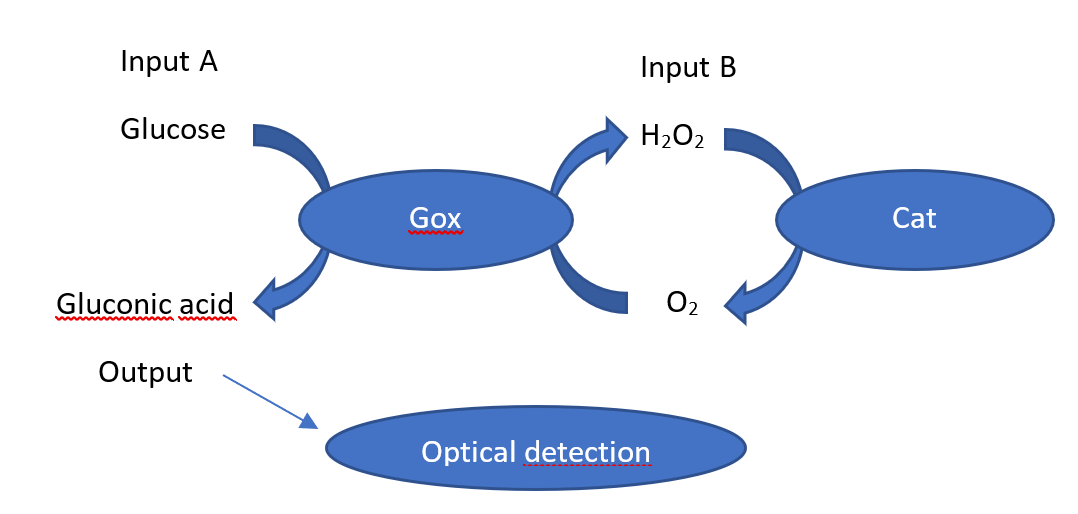
\includegraphics[scale= 0.33]{pics/ANDneu.png} \caption{A combination of chemical inputs and enzymes mimicking the Boolean gate AND} \label{img:and} \end{figure}
		
		\begin{center}
		\begin{tabular}{c|c|c}
			Glucose & H\textsubscript{2}O\textsubscript{2} & Output\\\hline
			0 & 0 & 0\\ 
			0 & 1 & 0\\
			1 & 0 & 0\\
			1 & 1 & 1
		\end{tabular}
		\end{center}
	
\subsection{Networks with electrochemical transduction}

		By assembling multiple logic gates, each mimicking a Boolean operation, it is possible to create small logic networks (e.g. half-adder/half-subtractor). To convert the physical change of the final network output into an electric signal a transducer is added.
	
		\subsubsection{Network resulting in pH changes} The following exemplifies a network, composed of different enzyme-based logic gates, functioning as AND or OR. The cascade of reactions within that network, when all four input chemicals are present, results in pH changes. pH measures the degree to which a solution is acidic or alkaline. The scale is defined from 0 (acid solution) to 14 (lye solution)\cite{chemie2}. The logic network is composed of four concatenated logic gates. Those gates contain the enzymes alcohol dehydrogenase (ADH, disassembling toxic alcohols), glucose dehydrogenase (catalyst for the oxidation of glucose) and glucose oxidase\cite{chemie2}. The four specific different input signals are NADH (resulting through reduction from Nicotinamide-Adenine-Dinucleotide NAD, which is a coenzyme found in all living cells),  acetaldehyde (also named ethanal, which is an organic chemical compound, for example naturally occuring in coffee, bread, and ripe fruit), glucose and oxygen (O\textsubscript{2})\cite{chemie2}.
	 	When all inputs are present the reaction yields to an acid medium, lowering the original pH value of the solution from initially 6-7 to approximately 4. \cite{original}\cite{chemie}
	%erst kombination von reaktionen

		
		\begin{figure}
			\centering 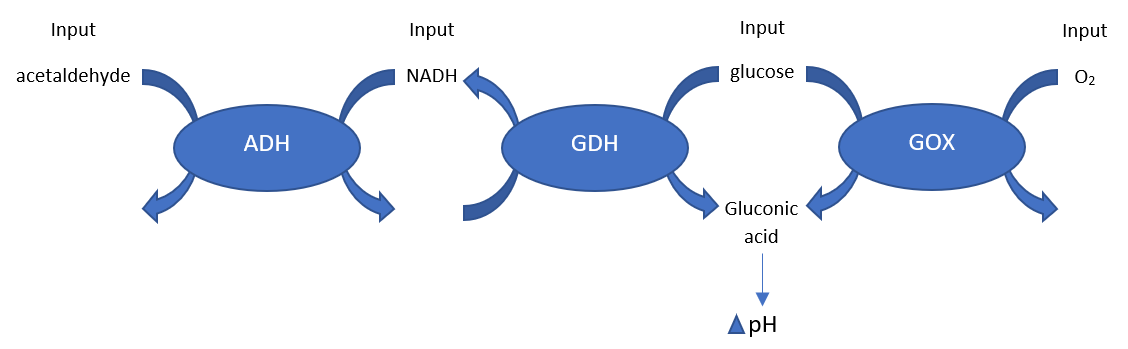
\includegraphics[scale= 0.35]{pics/network1.png}
			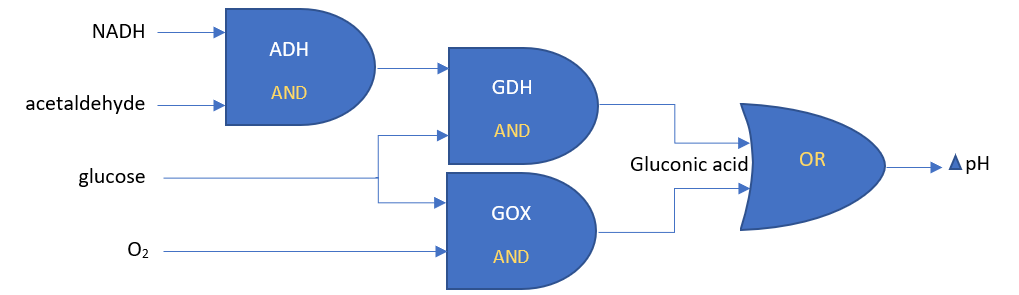
\includegraphics[scale = 0.39]{pics/network2.png} \caption{Network, composed of enzyme-based logic gates} 
		\end{figure}		
	%verbindung mit transducer
		
		\noindent The lowering of the pH value causes an electrochemical interface to switch from a preset OFF state to an ON state. 
		The interface is constructed to experience voltage changes according to the pH level. This interface functions as a transducer that makes the pH change electrochemically readable (therefore a low voltage marks the 0-value and a defined higher voltage the 1-value). While 16 different combinations of input signals are possible (being present or absent) only five of those resulted in an ON state and a significant high voltage. \cite{original}
		
		\begin{figure}[H] \centering \includegraphics[scale= 0.37]{pics/pH.png} \caption{Inputs/Voltage} \label{img:ph} \end{figure}
	
	

\section{Designing for biomedical analytic applications}
	To recognize various medical relevant conditions, it is necessary to use characteristic biochemical substances as inputs for the logic network.
	Physiological conditions resulting of an injury lead to a change in the concentration of some biochemical substances in the body that are typical for this condition. These substances can be used as inputs for the enzyme-based network created for the analysis.
	
	
	\subsubsection{Brain injury and hemorrhagic shock}
	
	The following logical system, composed of AND and IDENTITY gates, has been designed to process information related to brain injuries and hemorrhagic shock.
	The logic gates include the three enzymes lactate oxidase (can be used for the detection of lactate), horseradish peroxidase (an enzyme that is found in the roots of horseradish; extensively used in biochemistry applications)\cite{horse} and glucose dehydrogenese (a catalyst for the oxidation of glucose)\cite{chemie}.
	As inputs it receives the three substrates glucose, lactate (an ester or salt of lactic acid) and norepinephrine (a neurotransmitter) related to conditions originating from traumatic brain injury and hemorrhagic shock (a shock in which severe blood loss leads to inadequate oxygen delivery at the cellular level)\cite{shock}.\\
	An increased glucose concentration could relate to a hemorrhagic shock, while a higher lactate concentration could either indicate a hemorrhagic shock or a brain trauma and norepinephrine can be indicative of any traumatic injury. For the inputs, 0 has been defined with the normal physiologically concentration and 1 as an abnormally increased concentration. The two substrates norepiquinone (a biochemical product of the reaction between hydrogen peroxide and norepinephrine) and NADH that can result out of the reaction in the network, are measured by optical and electrochemicals means\cite{chemie2}. Especially the following combinations of input signals producing different combinations of NADH and norepiquinone appeared to correspond to the two different conditions. \cite{original}\cite{medicalapp}
	\vspace*{1cm}
	
	\begin{center}
		\begin{tabular}{l|>{\columncolor[gray]{0.8}}c|>{\columncolor[gray]{0.8}}c|c|c|c|}
			condition & norepiquinone & NADH & glucose & lactate & norepinephrine\\ \hline
			traumatic brain injury & 1&0&0&1&1\\
			hemorrhagic shock & 1&1 &1&1&1\\
		\end{tabular}
	\end{center}

	\vspace*{2cm}
	
\newpage
\section{Considerations}

Being only a concept yet, there are plenty of challenges that must be solved until a successful realization of complex applicable biosensors. The most current are as follows:

\subsubsection{Surface confinement}	In recent research, the success of enzymatic reactions was growingly dependant on the immobilization of the reagent layer. Early experiments with enzyme logic dissolved the gate constituents and chosen inputs in a solution. With the aim of complex networks that require multiple different gate constituents and inputs, each section needs to be differentiated and isolated, to prevent cross-reactions. To achieve multiple and combinable logic gates, the biocomputing layer needs to be immobilized. Agglomerations of multiple logic gates also induce further challenges. All reacting components need to be carefully evaluated to prevent cross-reactions, while the outside coating of the device must simultaneously protect the reagents within the device but be permeable to the desired inputs. The impact of an immobilization on the performance of biosensing devices has yet to be examined. \cite{original}

\subsubsection{Optimal transduction} With an increasing complexity of logic networks, the transduction of multiple outputs of the biocomputing layer becomes challenging. The current transducing solution is not capable of processing multiple output signals. It is highly desired to develop a solution that works with a single electrode. To efficiently scan for multiple output signals simultaneously, researchers hope to develop a single multipurpose catalytic layer to enhance the transduction and simplify the device. \cite{original}

\subsubsection{Defining the Boolean 0- and 1-values} For the biochemical logic networks as well as for the transductors, there have to be defined 0 and respectively defined 1 values. 0 should mark the biological standard value, while the state of the art is to define it as an absolute zero value. The definition of the 1-value is also problematic. In research, the 1 value has mostly been defined as a random convenient value, instead of using applicable medically critical values. Within the same field, the difference between a relevant 0 and a relevant 1 can be minimal. This leads to difficulties with the transduction accuracy. An offered solution would be a sigmoidal signal translation rather than the usual linear one, to emphasise the difference and allow a more reliable reading. 

\subsubsection{Scalability}	One central aim of research is to achieve a maximal flexibility of sensors. Ultimately it is highly desired to be able to scale every parameter of the sensor, from the complexity of the logic system to the specificity of the transducer. The potential to combine any given number of logic gates into networks which create increasingly complex logic systems is not yet achieved. 

\subsubsection{Relevant inputs}	A majority of laboratory projects worked with biomedically irrelevant substances for their proof of concept. An important step is to translate the working concept to applicable and relevant devices. In recent studies, scientists realized networks with biomedical relevant substances as inputs. The used logic networks yet did not depict a senseful logic context to the substances. Thus not only the work with relevant substances needs to be developed further, but also the logic networks need to be adjusted to depict relevant contexts. 

\subsubsection{Challenges of drug delivery}	One rather distant concern is the functionality of drug delivery devices. One of the key goals of research is to develop autonomous devices that analyse certain physiological parameters and offer an immediate reaction. Experiments have shown a need for different methods and technology to distribute the correct treatment within the cycle of those devices. \cite{original}


\section{Conclusion}

The concept of enzyme-based digital biosensing devices promises great scientific progress. The biggest hopes lay on the possible medical applications, while fields like homeland security and food safety also see great potential in the technology. Concurrently, the state of the art research is far from presenting any applicable devices. Most papers concentrate on proof of concept and define at least as many further challenges as they produce progress. To reach the desired heights, professionals from biochemistry, computer science and engineering will have to go to great lengths. But if the technology can only deliver half of what it promises, the effort might be worth it.


\newpage

\begin{thebibliography}{8}
	\bibitem{chemie}
	Frederic Barrière, Dónal Leech, Marie Pellissier: Powering fuel cells through biocatalysis. In: Electrochemical Sensors, Biosensors and their Biomedical Applications (2008), pp. 385-410. URL: https://doi.org/10.1016/B978-012373738-0.50014-3, last accessed 27 June 2018
	
	\bibitem{chemie2}
	Uwe Bornscheuer, Alfred P{\"u}hler (editors): R{\"o}mpp-Kompakt-Lexikon Biochemie und Molekularbiologie (2000). Thieme-Verlag, Stuttgart
	
	\bibitem{shock}
	Jeremy W. Cannon: Hemorrhagic Shock. In: The New York Journal of Medicine (2018). URL: M.D.https://www.nejm.org/doi/full/10.1056/NEJMra1705649, last accessed 22 June 2018
	
	\bibitem{definitions}
	Richard A. Durst, Daniel R. Thevenot, Klara Toth, George S. Wilson: Electrochemical biosensors: recommended definitions and classifications. In: Biosensors and Bioelectronics 16 (2001), pp. 121-131. URL:https://www.sciencedirect.com/science/article/pii/S0956566301001154, last accessed 27 June 2018
	
	\bibitem{haupt}
	Evgeny Katz: Enzyme-Based Logic Gates and Networks with Outout Signals Analyzed by Various Methods. In: ChemPhysChem 16 (2017), vol. 18, pp. 1688-1713. URL: https://onlinelibrary.wiley.com/doi/full/10.1002/cphc.201601402, last accessed 1 July 2018
	
	\bibitem{medicalapp} 
	Evgeny Katz, KM Manesh, Josef Wang and others: Enzyme logic gates for the digital analysis of physiological level upon injury. In: Biosens Bioelectron (2009). URL: https://www.ncbi.nlm.nih.gov/pubmed/19523809, last accessed 25 June 2018
	
	\bibitem{original}
	Evgeny Katz, Joseph Wang: Digital biosensors with build-in logic for biomedical applications - biosensors based on a biocomputing concept, In: Anal. Bioanal. Chem. (2010), pp. 1591-1603 
	
	\bibitem{application review}
	Parikha Mehrotra: Biosensors and their applications - A Review (2016). URL: https://www.ncbi.nlm.nih.gov/pmc/articles/PMC4862100/. Last accessed 26 June 2018
	
	\bibitem{state of the art}
	Shengbo Sang, Wendong Zhang and Yuan Zhao: State of the Art in Biosensors. In: State of the Art of Biosensors (2013), pp. 89-110. URL: https://www.intechopen.com/books/state-of-the-art-in-biosensors-general-aspects/review-on-the-design-art-of-biosensors, last accessed 1 July 2018
	
	\bibitem{horse}
	Nigel C. Veitch: Horseradish peroxidase: a modern view of a classic enzyme. In: Phytochemistry
	Volume 65 (2004), pp. 249-259 
	URL: https://www.sciencedirect.com/science/article/abs/pii/S0031942203006551  Last accessed 22 June 2018
	

	
\end{thebibliography}
\end{document}
